\clearpage
\begin{flushright}
	\textit{Лекция №6}
	\textit{2015.09.22}
\end{flushright}

\section{Системный вызов wait()}

Переводит процесс в состояние ожидание. Предназначен для перевода процесса-предка в состояние ожидания завершения своих потомков. 

Если в \ref{listing:fork} в родителя поставить wait(\&status), то предок будет ждать завершение потомков. 
Процессы зомби – специально введённое состояние процесса. Все процессы проходят это состояние. 

\begin{figure}[H]
	\centering
	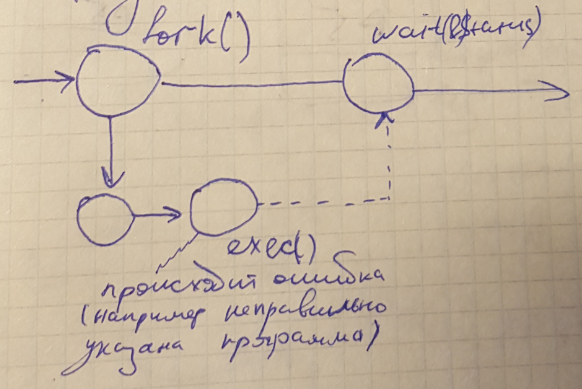
\includegraphics[width=\textwidth]{pic/4.png}
	\caption{Бесконечная блокировка на wait}
\end{figure}

Процесс предок бесконечно блокирован на wait, если потомок уже завершился, до вызова wait.

Процесс при завершении получает статус зомби, в системе помечается буквой Z, до момента, пока процесс не вызовет системный вызов wait.  Зомби – процесс, у которого отобраны все ресурсы, кроме строки в таблицы процессов (дескриптор). 

\section{Группы процессов (сигналы)}

В Unix процессы объединяются в группы. Главная группа – терминальная. Любой предок, вызвавший потомков, создает группу процессов. Объединение в группы для того, чтобы процессы одной группы могли получать одни и те же сигналы.
В Unix - сигналы, в Windows – события. Механизм сигналов в Unix позволяет процессам реагировать на события, которые могу произойти или внутри самого процесса или вне его. Сигнал – базовое средство информирования процессов о событиях в системе.
Самым важным событием в системе является завершение процесса. Получение процессом сигнала указывает ему на необходимость завершиться.  Вместе с тем, реакция процесса на принимаемый сигнал зависит от того, как сам процесс определил свою реакцию на данный сигнал. Для этого процесс должен содержать свой обработчик сигнала, если процесс желает изменить реакцию на получаемый сигнал, он должен определить эту реакцию с помощью своего обработчика сигнала. В классических системах сигналов не может быть больше 20. Для удобства каждый сигнал имеет цифровой идентификатор и буквенный. Все значения сигналов хранятся в файле \verb|signal.h|. 
Сигналы относятся к IPC. Рассматриваем для того, чтобы закруглить отношение о процессах. Если затрагиваем группы процессов, то нужно затронуть сигналы. 

\begin{figure}[H]
	\centering
	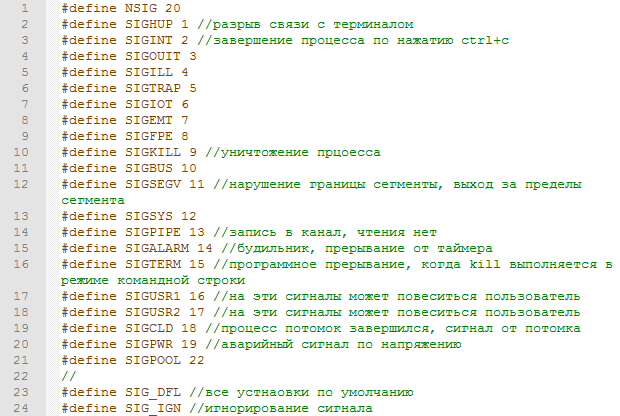
\includegraphics[width=\textwidth]{pic/5.png}
	\caption{Сигналы}
	\label{listing:signals}
\end{figure}

В \ref{listing:signals} \#3 это клавиша $QUIT$ или $ctrl + / $
Средством приема и посылки сигналов является системные вызовы \verb|kill()| и \verb|signal()|.

\subsection{Системный вызов kill()}.

Предписывает уничтожение процесса.  
\verb|kill(pid, sig)|. Сигнал будет послан всем процессам. Если pid <= 1, то сигнал будет послан группе процессов. Если pid равен 0, то sig посылается каждому процессу, который входит в группу текущего процесса. Если pid = -1,  то сигнал будет послан процессам, которых user id такой же, как и у процесса, который вызвал kill. 

\subsection{Системный вызов signall()}.
идентифицирует сигнал и воспринимает сигнал. Реакции процесса на системный вызов signal с аргументом func будет вызов функции func() . Процесс имеет возможность определить с помощью функции собственную реакцию на получаемый сигнал. 

\chapter{Управление памятью}

Подразумевается управление ОЗУ. В системе имеется иерархия памяти, рассматривается в зависимости от близости к процессору. ПРОЦЕССОР СВОЕЙ ПАМЯТИ НЕ ИМЕЕТ. В кристале процессора три кеша: данных, команд, TLB (прим. ред. специализированный кэш центрального процессора, используемый для ускорения трансляции адреса виртуальной памяти в адрес физической памяти.).

\begin{table}[H]
\caption{Иерархия памяти}
\begin{tabular}{|l|}
\hline
Внешнее ЗУ\\
\hline
ОЗУ\\
\hline
КЭШ 1-го уровня\\
\hline
Процессор\\
\hline
\end{tabular}
\end{table}

Вертикальное – передача данных с уровня на уровень. Горизонтальное управление – управление ???. Внешним ЗУ управляет файловая система. Файловая система обеспечивает доступ к хранимой информации. 

\paragraph{ОС однопрограммная пакетной обработки}
Всё адресное пространство ОЗУ отдано одной единственной программе. Но на самом деле 2 программы: ОС и программа. С помощью регистра границы (куда записывается адрес ОС) ОС защищается от программы.

\begin{figure}[H]
	\centering
	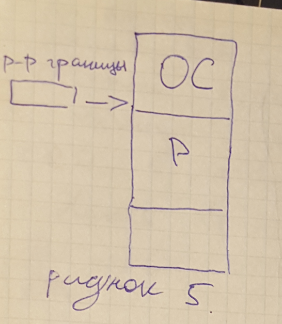
\includegraphics[width=\textwidth]{pic/6.png}
	\caption{ОС однопрограммная пакетной обработки}
\end{figure}

Идея ДОСа – как можно меньше места в ОЗУ. 

\begin{table}[H]
\caption{Дос}
\begin{tabular}{|l|l|}
\hline
0Мб & Резидентная часть  (не можем выгрузить)\\
\hline
& Резидентные программы\\
\hline
& Собственные сегменты программы\\
\hline
& Динамическая память. Её размер – динамически меняется.\\
\hline
& Транзитная часть (по мере необходимости вызывается в память\\
& Сейчас называется не подгружаемая страницы.\\
\hline
& резидентная часть\\
1Мб & \\
\hline
\end{tabular}
\end{table}

Резидент – шпион, постоянно находящийся в чужой стране.  DOS – однозадачная ОС, в памяти только одна программа. На самом деле – несколько программ: DOS, резидентные программы, программа. Память делится между ОС и приложением. Приложение не должно обращаться в некоторые важные области памяти. ДОС плохо защищенная ОС. Сегменты – перемещаемые. Одиночное непрерывное распределение памяти.

\paragraph{Мультипрограммные ОС}
Следующий этап развития ОС – мультипрограммные. Основная цель – сократить время переключения с одной программы на другую. 

\paragraph{Разделение памяти с фиксированным размером}

\begin{figure}[H]
	\centering
	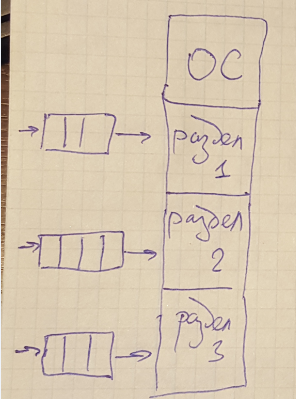
\includegraphics[width=\textwidth]{pic/7.png}
	\caption{разделение памяти с фиксированным размером}
\end{figure}

\paragraph{Разделами переменного размера}

\begin{figure}[H]
	\centering
	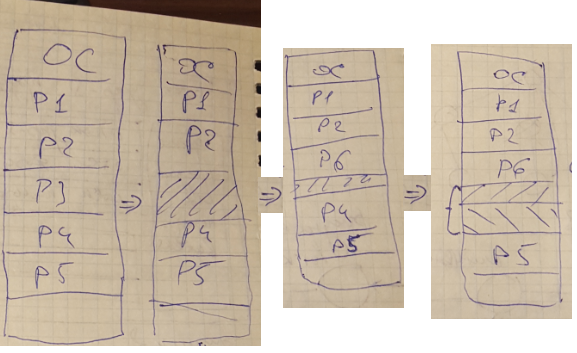
\includegraphics[width=\textwidth]{pic/8.png}
	\caption{разделами переменного размера}
\end{figure}

В начальный момент мы можем загрузить программы в последовательные адреса.
В результате освобождения и загрузки память будет фрагментированной.